\chapter{Related Work}
\label{related_work}
Motion planning is a widely researched topic with roots in control, artificial intelligence, computational geometry and Robotics. The literature presented in \cite{book_robot_motion_planning}, \cite{book_lavelle_planning} review significant portion of standard planning techniques. Due to the complexity of the autonomous cars and the environments, general techniques from robotics cannot be applied. Planning for autonomous cars in general is sub divided into two categories namely planning in unstructured environments such as parking areas etc and structured environments such as Road Networks where the traffic rules have to be followed. This chapter mainly focuses on the planning techniques in structured urban environments. 

\section{Planning Approaches}
\label{planning_aproaches}

Autonomous vehicles have been in research communities from 80's with projects such as PROMETHEUS \cite{prometheus}, the research was accelerated by the DARPA Grand Challenge in 2006 and DARPA Urban Challenge(DUC) in 2007 \cite{darpa_urban_challenge}. In DUC, six autonomous vehicles from different universities have completed the challenge and have used various techniques to accomplish the task. These techniques have formed the basis for modern day autonomous cars which perform much sophisticated compared to the DUC participants. 

Approach followed by different participants of DUC are described in \cite{darpa_urban_challenge}. Planning module of Boss, autonomous vehicle from Carnegie Melon University which won the DUC is described in general here. Its planning framework is mainly subdivided into 3 sub modules 

\begin{itemize}
	\item Mission control is the higher level module which creates a global path, assigns lane to the vehicle to reach the check points, detects blockades.
	\item Behavioral module is responsible for decisions such as precedence at intersections, lane change decision, speed planning, look ahead point assignment etc. 
	\item Motion planning module is responsible for generating local trajectories and converting them to steering and acceleration values. It initially creates a forward looking path and velocity planning is performed on top of that. 
\end{itemize}

After DUC, there has been a huge research into this accelerated by the industry because of benefits from autonomous driving. Planning for autonomous driving in general can be classified as shown in Figure \ref{related_work_classification}. The following sub sections discuss research in each of the described sub-categories. 

\begin{figure}[H]
	\centering
	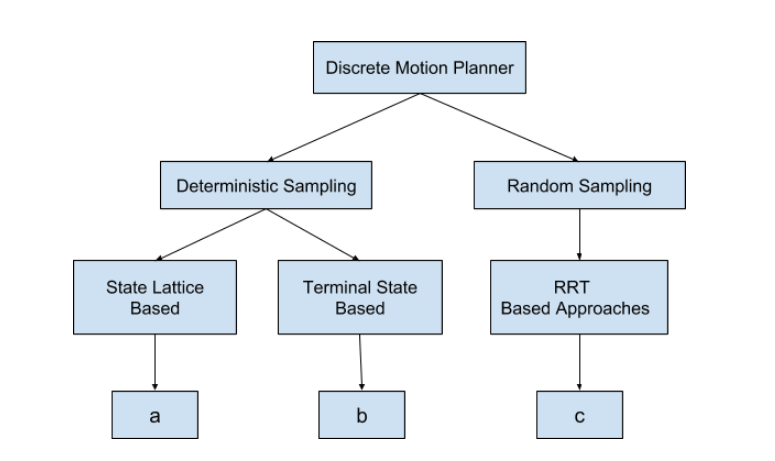
\includegraphics[width=0.8\textwidth]{Images/related_work/planning_division.png}
	\caption{General Overview of On-road planners. a - \cite{cmu_parallel_thesis}  \cite{diss_shui_phd_thesis} \cite{traj_planner_optimization} \cite{lattice_Gu_Tiyanu} \cite{unit_A_star} , b - \cite{kolski_thesis} \cite{real_time_traj_plan_article} \cite{darpa_urban_challenge}, c -\cite{rrt_star} \cite{rrt_urban_driv} \cite{mit_rrt}
	}
	\label{related_work_classification}
\end{figure}

\subsection{Incremental Search Approaches}
\label{rw_incremental_search}

different RRT approaches - start from MIT planner

RRT*

advantages and disadvantages of RRT

Check Davids thesis

\subsection{Lattice Planners}
\label{rw_lattice_planners}
The algorithm uses a discrete representation of the planning area with multiple states, often a multi dimensional one with dimensions such as position, acceleration, velocity, time etc. All of these states are connected together and the problem then reduces to finding a path from the initial state to the final state in the lattice. 

write different improvements in different planners proposed

howard intitial lattice 

werling et al - next

mcnought - cmu 

cmu traj optimization

diss shui planner 

Advantages and disadvanatages of Lattice 

\subsection{Local Search}
\label{rw_local_search}

Local Search or forward projecting trajectories
Different types of curves, 
forward samples, 


Velocity planning some where

sampling
Action space - something similar to this thesis, 
State Space - final states

Combining Path and Velocity
Werling, Lattices do that


%\subsection{Sampling Approaches}
%\label{sampling}



%\subsection{Trajectory Representation}
%\label{trajectory_rep}
%splines? polynomials? lattice?


\section{Trajectory Evaluation}
\label{traj_eval}
collison checking, cost functions for different things


\section{Evaluation Criteria}


%Look if the sampling based, RRT based, lattice based etc etc should be combined together?
%write about MDP, POMDP etc 